\paragraph{Мейн}

Данный ELF исполняемый файл не запускался на моём компьютере из-за ошибок с библиотекой pyautogui и
отсутствия файла task\_4.py.
Для анализа использовался дизассемблер Ghidra.

\paragraph{Описание}
Программа task\_5 реализует загрузчик Python-приложения, упакованного с помощью PyInstaller.
Основная задача - извлечь необходимые файлы во временный каталог, настроить окружение Python и запустить приложение.

Ключевые компоненты и функциональность
\begin{itemize}
    \item Точка входа (processEntry)
    \begin{itemize}
        \item Вызывает \texttt{\_\_libc\_start\_main} для инициализации окружения.
        \item Передаёт управление основной функции \texttt{thunk\_FUN\_00403e50}
    \end{itemize}
    \item Основная функция \texttt{thunk\_FUN\_00403e50}
    \begin{itemize}
        \item Инициализация буферов и переменных
        \item Проверка переменных окружения:
        \begin{itemize}
            \item \texttt{\_MEIPASS2} - каталог с извлечёнными файлами
            \item \texttt{\_PYI\_ONEDIR\_MODE} - режим работы PyInstaller
            \item \texttt{\_PYI\_PROCNAME} - имя процесса Linux (устанавливается через prctl)
        \end{itemize}
    \end{itemize}
    \item Функция инициализации \texttt{FUN\_004086c0} - Конструктор, выполняющий \texttt{\_\_DT\_INIT\_ARRAY}
    до запуска основной функции
    \item Основные функции загрузчика
    \begin{itemize}
        \item Управление архивом PyInstaller
        \item Управление переменными окружения
        \item Обработка ошибок
        \item Управление памятью и очистка временных ресурсов
    \end{itemize}

\end{itemize}

\paragraph{Тестовый запуск}
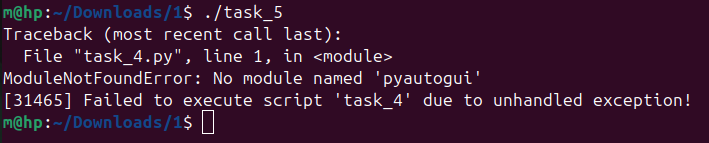
\includegraphics[width=1\linewidth]{static/_task_5}
